%!TEX root = Thesis.tex

\chapter{State of the art}
\label{chapter:stateofart}

% Na reunião em do feedback do relatório tinha-se falado em ter o overview do EAC no capítulo de nomenculatura e conceitos de clustering (que também irá incluir o K-Means e o single link). No entanto, tendo que estes dois algorithmos são "clássicos" e o EAC é state-of-the-art não faria sentido ter a explicação do EAC logo no inicio do capítulo State of the Art?

% A ideia seria então começar por explicar o EAC. Depois disso, rever o que foi feito em termos de escalibilidade do mesmo. Depois ter uma secção de Big Data em que basicamente se mostraria o que pode ser feito nesta área (ou talvez ter esta secção antes da escalibilidade do EAC). E só depois poria as secções do quantum clustering e do conceito e algoritmos GPU.


% motivation
Scalability of EAC to large data sets is the concern of this work and, because of that, this chapter starts by reviewing what has been done in terms of scaling EAC in section \ref{sec:eac scaling}.
EAC is a method of three parts and this dissertation is concerned with the scalability of the whole algorithm which means that each step must be optimized.
Scaling an algorithm means one has to take into account both speed of execution and memory requirements.
Increasing speed can be attained with either faster algorithms and/or faster computation of existing algorithms.
% Both these approaches to faster generation of the ensemble were pursued and researched.
This chapter reflects research done within both approaches.

% EAC section
% Before reviewing methods and techniques relevant for scaling EAC, this chapter starts by presenting the state of the art of EAC and related research in section \ref{sec:eac}.
% This section provides a brief overview of ensemble clustering, explains the EAC algorithm, refers to where it has been applied and reviews what has been done in terms of scaling it.

% large datasets section
Although research on the application of EAC to large data sets has not been pursued before, cluster analysis of large data sets has. 
Since EAC uses traditional clustering algorithms (e.g. K-Means, Single-Link) in its approach, it is useful to understand how scalable the individual algorithms are as they will have a big impact in the scalability of EAC.
Furthermore, valuable insights may be taken from the techniques used in the scalability of other algorithms.
To this end, section \ref{sec:big data} presents a brief review on cluster analysis of large data sets, with a focus on parallelization with GPUs.
Furthermore, it offers a more detailed description of a GPU parallel version of K-Means and an approach for parallelizing Single-Link with the GPU.

% quantum clustering
An alternate approach on clustering for scaling with faster algorithms, the still young field of quantum clustering, was reviewed in section \ref{sec:quantum clustering}.
This line of research was taken mostly with the first step of EAC in mind.


% The former in the form of the still young field of quantum clustering, which is briefly reviewed in section , and the latter in the field of parallel computation, more specifically on computation in GPUs, reviewed in section \ref{sec:gpgpu}.
% While quantum clustering was only reviewed for the first step, the parallel computation paradigm was investigated with all steps in mind.
% For that reason, K-Means GPU versions were researched as well as a MST-based Single Linkage Clustering method.

% % % % % % % % % % % % % % % % % % % % % % % % % % % % % % % % % % % % % % % %
%
%  					EAC SCALABILITY
%
% % % % % % % % % % % % % % % % % % % % % % % % % % % % % % % % % % % % % % % %


\section{Scalability of EAC}
\label{sec:eac scaling}
The quadratic space and time complexity of processing the $n \times n$ co-association matrix is an obstacle to an efficient scaling of EAC.
Two approaches have been proposed to address this obstacle: one dealing with reducing the co-association matrix by considering only the distances of patterns to their $p$ neighbors and the other by using a sparse co-association matrix and maximizing its sparsity.

\subsection{$p$ neighbors approach}
The first approach, \cite{Fred2005}, proposes an alternative $n \times p$ co-association matrix, where only the $p$ nearest neighbors of each pattern are considered in the evidence combination step.
This comes at the cost of having to keep track of the neighbors of each pattern in a separate data structure of $O(np)$ memory complexity and also of pre-computing the $p$ neighbors, which has a time complexity of $O(n^2)$ to compute the similarity measure from each pattern to every other pattern.
The quadratic space complexity of the co-association matrix is then transformed to $O(2np)$: $O(np)$ for the actual co-association matrix and $O(np)$ for keeping track of the neighbors.
Since usually one has $p < \frac{n}{2}$ (value for which both this approach and the original $n \times p$ matrix would take the same space), the cost of storing the extra data structure is lower than that of storing an $n \times n$ matrix, e.g. for a dataset with $10^6$ patterns and $p=\sqrt{10^6}$ (a value much higher than the $20$ neighbors used in \cite{Fred2005}), the total memory required for the co-association matrix would decrease from $3725.29 GB$ to $7.45 GB$ ($0.18\%$ of the memory occupied by the complete matrix).
% However, it should be noted that computing the $p$ nearest neighbors requires the computation of $n^2$ distance values.

\subsection{Increased sparsity approach}
The second approach, presented in \cite{Lourenco2010}, exploits the sparse nature of the co-association matrix.
The co-association matrix is symmetric and with a varying degree of sparsity.
The former property translates in the ability of storing only the upper triangular of the matrix without any loss on the quality of the results.
The latter property is further studied with regards to its relationship with the minimum $K_{min}$ and maximum $K_{max}$ number of clusters in the partitions of the input ensemble.
The core of this approach is to only store the non-zero values of the upper triangular of the co-association matrix.
The authors study 3 models for the choice of these parameters:

\begin{itemize}
	\item choice of $K_{min}$ based on the minimum number of gaussians in a gaussian mixture decomposition of the data;
	\item based on the square root of the number of patterns ($\{K_{min},K_{max}\} = \{\frac{\sqrt{n}}{2},\sqrt{n}\}$);
	\item or based on a linear transformation of the number of patterns ($\{K_{min},K_{max}\} = \{\frac{n}{A},\frac{n}{B}\},A<B$).
\end{itemize}

where $A$ and $B$ are two suitable constants chosen by the researcher.
The study compared the impact of each model in the sparsity of the co-association matrix (and, thus, the space complexity) and in the relative accuracy of the final clusterings.
Both theoretical predictions and results revealed that the linear model produces the highest sparsity in the co-association matrix, under a dataset consisting of a mixture of Gaussians.
Furthermore, it is true for both linear and square root models that the sparsity increases as the number of samples increases.

For real data sets, the performance of the three models became increasingly similar with the increase of the cardinality of the problem.
It was found that the chosen granularity of the input partitions ($K_{min}$) is the variable with most impact, affecting both accuracy and sparsity.
The authors reported this technique to have linear space and time complexity on benchmark data.

The number of samples of the data sets analysed in \cite{Lourenco2010} was under $10^4$.
Furthermore, it should be noted that the remarks concerning the sparsity of the co-association matrix in the aforementioned study refer to the number of non-zero elements in the matrix and does not take into account extra data structures that accompany real sparse matrices implementations.

% Although the results appear promising, the present work aims to deal with datasets much larger than this and, as a consequence, this technique should be further evaluated and tested to attest to its usefulness to very large datasets. %TODO: this paragraph is probably more relevant in the methodology section so as to introduce why other techniques were necessary


% % % % % % % % % % % % % % % % % % % % % % % % % % % % % % % % % % % % % % % %
%
%  					BIG DATA CLUSTERING
%
% % % % % % % % % % % % % % % % % % % % % % % % % % % % % % % % % % % % % % % %

\section{Clustering with large datasets}
\label{sec:big data}

% \subsection{The concept of Big Data}
% % there is a difference between this and the big data section in the state of the art chapter
% % here we are dealing with the big data paradigm, an overview of what is, what has been happening
% % I'm trying t justigy why big data is an interesting 
% % most focus should into the problems themselves and why they are interesting

% examples of success application

% characteristics and challenges
% \subsection{Computation in Big Data}

% this is probably good for motivating this section in the introduction of the chapter
% Scalability of EAC within the big data paradigm is the concern of this work.
% Although this line of research has not been pursued before, cluster analysis of large data sets has.
% Since EAC uses traditional clustering algorithms (e.g. K-Means, Single-Link) in its approach, it is useful to understand how scalable the individual algorithms are as they will have a big impact in the scalability of EAC.
% Furthermore, valuable insights may be taken from the techniques used in the scalability of other algorithms.


%this was taken from the Data Clustering: Algorithms and Applications book

% introcution for big data clustering
When large datasets, and big data, is in discussion, two perspectives should be taken into account \cite{Aggarwal2014}.
The first deals with the applications where data is too large to be stored efficiently.
This is the problem that streaming algorithms such as LOCALSEARCH \cite{bigdatastream} try to solve by analyzing data as it is produced, close to real-time processing.
The other perspective is data that is actually stored for later processing which is the perspective relevant to the present work and will be further discussed below.

% different approaches on big data clustering
The flow of clustering algorithms typically involves some initialization step (e.g. choosing the number of centroids in K-Means) followed by an iterative process until some stopping criteria is met, where each iteration updates the clustering of the data \cite{Aggarwal2014}.
In light of this, to speed up and/or scale up an algorithm, three approaches are available: (1) reduce the number of iterations, (2) reduce the number of patterns and/or features to process or (3) parallelizing and distributing the computation.
The solutions for each of this approaches are, respectively, one-pass algorithms (e.g. CLARANS \cite{ng2002clarans}, BIRCH \cite{zhang1996birch}, CURE \cite{guha1998cure}), randomized techniques that reduce the input space complexity (e.g. PCA, CX/CUR \cite{drineas2006fast}) and parallel algorithms (parallel K-Means \cite{Zechner2009b}, parallel spectral clustering \cite{chen2011parallel}).

% another example for randomized techniques that reduce input space complexity: local-preserving projection \cite{johnson1984extensions};
% CX/CUR is a global projection

% parallelization approach to big data clustering
Parallelization can be attained by adapting algorithms to multi core CPU, GPU, distributed over several machines (a \emph{cluster}) or a combination of the former, e.g. parallel and distributed processing using GPU in a cluster of hybrid workstations.
Each approach has its advantages and disadvantages.
% CPU
The CPU approach has access to a larger memory but the number of computation units is reduced when compared with the GPU or cluster approach.
Furthermore, CPUs have advanced techniques such as branch prediction, multiple level caching and out of order execution - techniques for optimized sequential computation.
% GPU
GPU have hundreds or thousands of computing units but typically the available device memory is reduced which entails an increased overhead of memory transfer between host (workstation) and device (GPU) for computation of large datasets.
In addition, it is harder to scale the above solutions for even bigger datasets.
On the other hand, GPUs can be found on a large variety of computing platforms, from mobile devices to workstations and datacenters.
% clusters
A cluster offers a parallelized and distributed solution, which is easier to scale.
According to \cite{Aggarwal2014}, the two algorithmic approaches for cluster solutions are (1) memory-based, where the problem data fits in the main memory of the machines of the cluster and each machine loads part of the data; or (2) disk-based, comprising the widely used MapReduce framework capable of processing massive amounts of data in a distributed way.
The main disadvantage is that there is a high communication and memory I/O cost to pay.
Communication is usually done over the network with TCP/IP, which is several orders of magnitude slower than the direct access of the CPU or GPU to memory (host or device).

% overview of the section; motivation for GPU K-Means and GPU SL/MST
The present work is oriented towards GPU based parallelization, since GPUs are an easily accessible commodity and the goals of the dissertation are oriented towards computation on a single machine.
Taking that into consideration, this section starts by covering a review of the General Purpose computing on GPUs paradigm.
It goes on to review a GPU parallel version of the K-Means algorithm and a GPU parallel approach for performing Single-Link clustering.

\subsection{General Purpose computing on Graphical Processing Units}
\label{sec:gpgpu}

The original intended used for GPUs was graphics processing, hence its name.
Recently, GPUs have been increasingly used for other purposes - a trend commonly known as General Purpose processing in Graphics Processing Units (GPGPU).
%Using GPU for other applications other than graphic processing, commonly known as GPGPU, has become a trend in recent years.
GPU present a solution for "extreme-scale, cost-effective, and power-efficient high performance computing" \cite{Chen2012}.
Furthermore, GPU are typically found in consumer desktops and laptops, effectively bringing this computation power to the masses.

GPUs were typically useful for users that required high performance graphics computation.
Other applications were soon explored as users from different fields realized the high parallel computation power of these devices.
However, the architecture of the GPUs themselves has been strictly oriented toward the graphics computing until the appearance of specialized GPU models designed for data computation (e.g. NVIDIA Tesla).

GPGPU application on several fields and algorithms has been reported with significant performance increase, e.g. application on the K-Means algorithm \cite{Bai2009,Wu2011,Zechner2009,Wu2009a}, hierarchical clustering \cite{Shalom2009,ArulShalom2011}, document clustering \cite{gao20xx}, image segmentation \cite{Sirotkovi2012}, integration in Hadoop clusters \cite{Malakar2013,Grossman2013}, among other applications.

%TODO add refs for energy
Current GPUs pack hundreds of cores and have a better energy/area ratio than traditional infrastructure.
GPU work under the SIMD framework, i.e. all the cores in the device execute the same code at the same time and only the data changes over time.

\subsubsection{Programming GPUs}

% old part, i.e. shading models, DirectX, OpenGL, grahics pipeline
In the very beginning of GPGPU, programming was done directly through graphics APIs.
Programming for GPUs was traditionally done within the paradigm of graphics processing, such as DirectX and OpenGL.
If researchers and programmers wanted to tap into the computing power of a GPU they had to learn and use these APIs and frameworks, which is a challenging task since their general problems had to be modelled to the graphics-oriented primitives \cite{Misi2012}.
With the appearance of DirectX 9, shader programming languages of higher level became available (e.g. C for graphics, DirectX High Level Shader Language, OpenGL Shading Language), but they were still inherently graphics programming languages, where computation must be expressed in graphics terms. 

% new part, i.e. interest in GPGPU sparkled unified devices and frameworks
% overview of recent programming models, CUDA is computing framework, OpenCL is a standard
More recent programming models, such as CUDA and OpenCL, removed a lot of that burden by exposing the power of GPUs in a way closer to traditional programming.
Currently, the major programming models used for computation in GPU are OpenCL and CUDA.
While the first is widely available in most devices, the latter is only available for NVIDIA devices.

% give references for GPU MapReduce
As Google's MapReduce computing model has increasingly become a standard for scalable and distributed computing over big data, attempts have been made to port the model to the GPU \cite{Ji2011,Xin2012,He2008}.
This translates in using the same programming model over a wide array of computing platforms.


\subsubsection{OpenCL vs CUDA}
% TODO rewrite this on terms of a better comparisson NEEDS REFS

Presently, the most mature programming models are CUDA and OpenCL.
CUDA appeared first and is supported only by NVidia devices.
It is also the most mature of the two and performs well since it was designed alongside with the hardware architecture of the supporting devices.
OpenCL has the advantage of portability, but that comes with issues of performance portability.
Both models are, in fact, very similar and literature suggests that porting the code from one to the other requires minimal changes \cite{Karimi2010,Su2012}.
Literature also reports that CUDA performs better than OpenCL \cite{Su2012} for equivalent code.

% TODO CUDA and OpenCL comparison; they are very similar in lots of ways; languanges they support (Python, Java, C, Pascal,...)


% TODO performance portability problem, how the performance problem can be mitigated and even eliminated by careful choice of compiler parameters, device aware application and so on (Fang2011)


% TODO This should go for methodology
% In the end, the choice of GPU computing framework was CUDA.
% All the infrastructure available for developing and testing supports CUDA.
% Another reason for the choice is that all the work is being developed in Python and Python has a CUDA API of very high level - part of the Numba module developed by Continuum Analytics. 


\subsubsection{Overview of CUDA}

%TODO needs refs, it is mostly the C CUDA programming guide

This section presents an overview of the CUDA programming model and its main concepts and characteristics.
For a more thorough and extensive explanation of these topic, the CUDA C Programming Guides \cite{Nvidia2014}, the source of the present review, should be consulted.
A GPU is comprised by one or several streaming processors (or multiprocessor).
Each of this processors contains several simpler processors, each of which execute the same instruction at the same time at any given time.
In the CUDA programming model, the basic unit of computation is a \emph{thread}.
Threads are grouped into \emph{blocks} which are part of the block \emph{grid}.
The number of threads in a block is typically higher than the number of processors in a multiprocessor.
For that reason, the hardware automatically divides the threads from a block into smaller batches, called \emph{warps}.
This hierarchy is represented in Figure \ref{fig:gridthread}.
The computation of one block is independent from other blocks and each block is scheduled to one multiprocessor, which means that more multiprocessors results in more blocks being processed at the same time, as represented in Figure \ref{fig:blockprocessor}.

\begin{figure}[ht]
\centering
\begin{minipage}[b]{.45\textwidth}
	\centering
	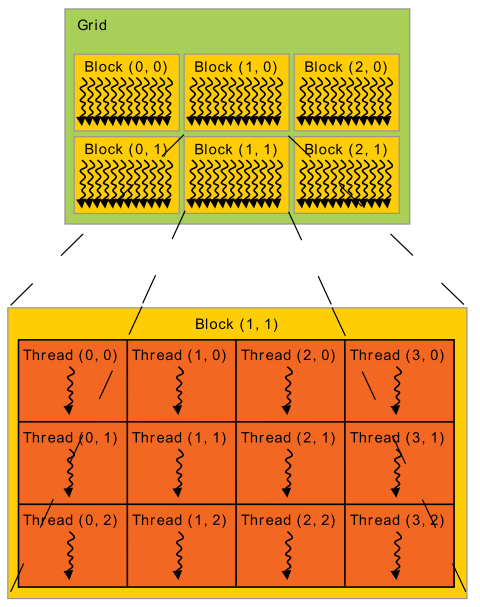
\includegraphics[width=.95\textwidth]{stateofart/gpgpu/threadgrid}
	\captionof{figure}{Thread hierarchy \cite{Nvidia2014}.}
	\label{fig:gridthread}  
\end{minipage}
\begin{minipage}[b]{.45\textwidth}
    \centering
    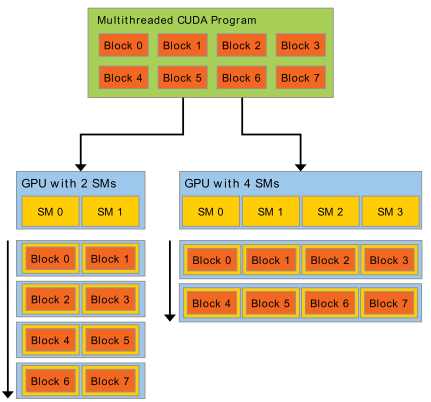
\includegraphics[width=.95\textwidth]{stateofart/gpgpu/blockprocessor}
    \captionof{figure}{Distribution of thread blocks is automatically scaled with the increase of the number of multiprocessors \cite{Nvidia2014}.}%Automatic scalability 
    \label{fig:blockprocessor}
\end{minipage}
\end{figure}

% \begin{figure}[!ht]
%     \centering
%     \begin{subfigure}[b]{0.45\textwidth}
%         \centering
%         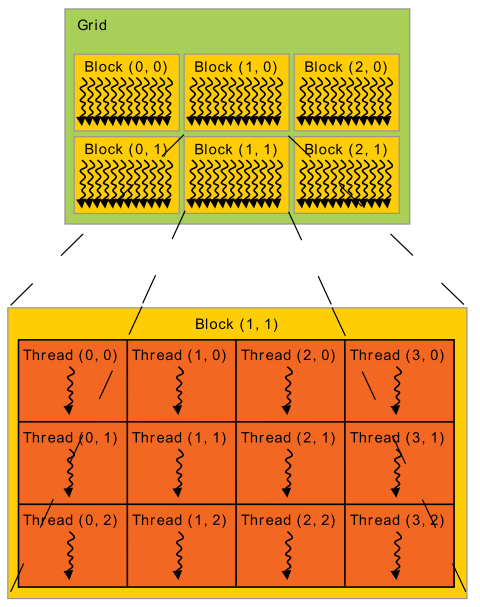
\includegraphics[width=\textwidth]{stateofart/gpgpu/threadgrid}
%         \caption{Thread hierarchy \cite{Nvidia2014}.}
%         \label{fig:gridthread}
%     \end{subfigure}
%     \hfill
%     \begin{subfigure}[b]{0.45\textwidth}
%         \centering
%         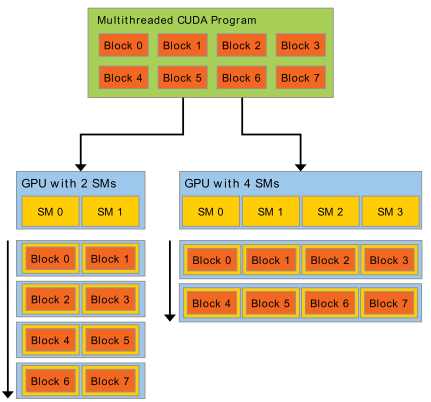
\includegraphics[width=\textwidth]{stateofart/gpgpu/blockprocessor}
%         \caption{Automatic scalability \cite{Nvidia2014}.}
%         \label{fig:blockprocessor}
%     \end{subfigure}
%     \caption{\ref{fig:gridthread} represents the thread hierarchy and \ref{fig:blockprocessor} shows how the distribution of thread blocks is automatically scaled with the increase of the number of multiprocessors.}
%     \label{fig:cuda fig1}
% \end{figure}

Block configuration can be multidimensional, up to and including 3 dimensions.
Furthermore, there is a limit to the amount of threads in each dimension that varies with the version of CUDA being used, e.g. for GPUs with CUDA compute capability 2.x  the number of threads is 1024 for the x- or y-dimensions, 64 for the z-dimension, an overall maximum number of threads is 1024 and a warp size of 32 threads.
For the previous example, it is wise for the number of threads used in a block to be a multiple of 32 to maximize processor utilization, otherwise some blocks will have processors that will do no work.

Depending on the architecture, GPUs have several types of memories.
Accessible to all processors (and threads) are the global memory, constant memory and texture memory, of which the last two are read-only.
Blocks share a smaller but significantly faster memory called shared memory, which is a memory inside a multiprocessor to which all processors have access to, enabling inter-thread communication inside a block.
Finally, each thread has access to local memory.
Local memory resides in global memory space and has the same latency for read and write operations.
However, if the thread is using only single variables or constant sized arrays, it uses register space to, which is very fast.
If the memory used exceeds the available register space the local memory used.
This memory hierarchy is represented in Figure \ref{fig:memorymodel}.

\begin{figure}[t]
\centering
\begin{minipage}[b]{.5\textwidth}
	\centering
	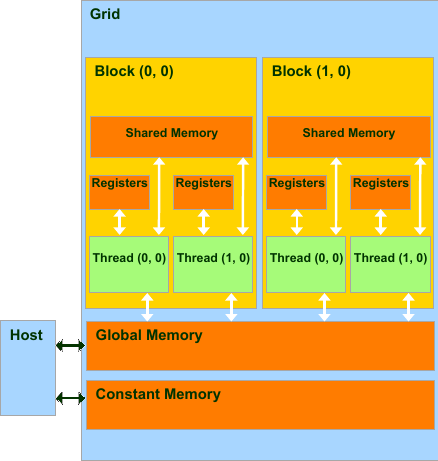
\includegraphics[width=0.9\textwidth]{stateofart/gpgpu/memorymodel}
	\captionof{figure}{Memory model used by CUDA \cite{Nvidia2014}.}
	\label{fig:memorymodel}  
\end{minipage}%
\begin{minipage}[b]{.5\textwidth}
        \centering
        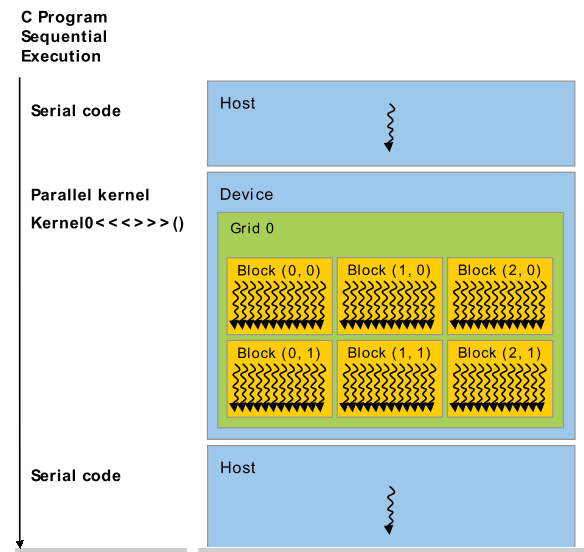
\includegraphics[width=0.9\textwidth]{stateofart/gpgpu/flow}
        \captionof{figure}{Sample execution flow of a CUDA application \cite{Nvidia2014}.}%Automatic scalability 
        \label{fig:cudaflow}
\end{minipage}
\end{figure}

% \begin{figure}[!ht]
%     \centering
%     % this was taken from the internet but is available at NVIDIA slides, could not find a decent reference
%     \begin{subfigure}[b]{0.45\textwidth}
%         \centering
%         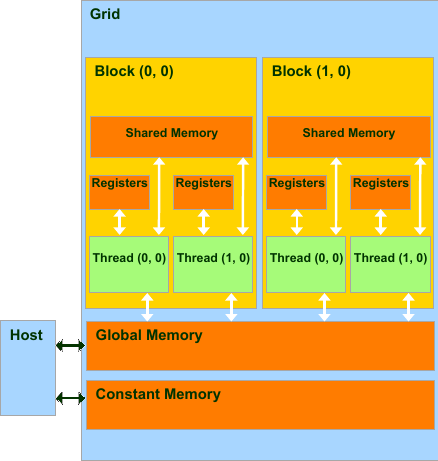
\includegraphics[width=\textwidth]{stateofart/gpgpu/memorymodel}
%         \caption{Memory model used by CUDA \cite{Nvidia2014}.}
%         \label{fig:memorymodel}
%     \end{subfigure}
%     \hfill
%     \begin{subfigure}[b]{0.45\textwidth}
%         \centering
%         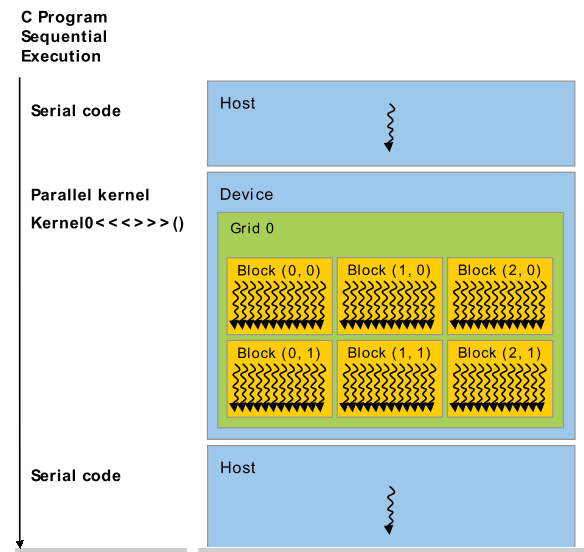
\includegraphics[width=\textwidth]{stateofart/gpgpu/flow}
%         \caption{Sample execution flow of a CUDA application \cite{Nvidia2014}.}
%         \label{fig:cudaflow}
%     \end{subfigure}
%     \caption{}
%     \label{fig:cuda fig2}
% \end{figure}

The typical flow of a CUDA application (and, typically, any modern GPU application) is explained in this paragraph and can be observed in Figure \ref{fig:cudaflow}.
First, the host CPU is responsible for several steps in the set-up phase.
The host starts by transferring any necessary to the device memory (global, texture or constant).
The next step is selecting the \emph{kernel} (the function that will run on the GPU processors) and the thread topology (configuration of threads in a block and blocks in the grid).
% First, the host CPU transfers any necessary data to the device memory (global, texture or constant) and is responsible for setting up the device code execution, which entails selecting the \emph{kernel} (the function that will run on the GPU processors) and the thread topology (configuration of threads in a block and blocks in the grid).
The set-up phase if followed by the computation phase in the GPU.
% The next phase is simply the device executing the kernel.
Finally, the host will transfer back the results from the device.
It should be noted that the latest architectures support \emph{Dynamic Parallelism}.
This functionality allows the device to start other kernels without the intervention of the host CPU, which would alter the typical execution flow explained above if used.
It can be particularly useful if several kernels have to be executed in an application from the same input data but with dependencies.
In such a scenario, a block of the second kernel could be executed as soon as all dependencies from the first kernel were met, effectively cutting overheads for kernel calling from the host CPU.


\subsection{Parallel K-Means}
\label{sec:parallel kmeans}

K-Means is an obvious candidate to generate the ensemble of the first step of EAC because it uses different initializations and parameters and due to its simplicity.
Besides, K-Means is a very good candidate for parallelization.
Still, other algorithms can be used to produce ensembles.

% As explained in chapter \ref{chapter:clustering}, K-Means has two main steps: labeling and update.

Several parallel implementations of this algorithm for the GPU exist \cite{Bai2009, Wu2011, Zechner2009, Sirotkovi2012, Farivar2008} and all report significant speed-ups relative to their sequential counterparts in certain conditions, usually after the input data set goes above a certain cardinality, dimensionality or number of clusters threshold.
The first step is inherently parallel as the computation of the label of the $i$-th pattern is not dependent on any other pattern, but only on the centroids.
Two approaches to parallelize this step on the GPU are possible, a centroid-centric or a data-centric \cite{Bai2009}.
In the former each thread is responsible for a centroid and will compute the distance from its centroid to every pattern.
These distances must be stored and, in the end, the patterns are assigned to the closest centroid.
In the latter, each thread will compute the distance from one or more data points to every centroid and determines to which centroid they are closest.
This strategy has the advantage of using less memory since it does not need to store all the pair-wise distances to perform the labeling - it only needs to store the best distance for each pattern.
According to \cite{Bai2009}, the former approach is suitable for devices with a low number of processors so as to stream the data to each one, while the latter is better suited to devices with more processors.

The approach taken in \cite{Zechner2009b} only parallelizes the labeling stage and takes a data-centric approach to the problem.
Each thread computes the distance from a set of data points to every centroid and determines the labels.
The remaining steps are performed by the host CPU.
This study reported speed ups up to 14, for input datasets of $500\:000$ points.
Furthermore, it should be noted that the speed up was measured against a sequential version with all C++ compiler optimizations turned on, including vector operations (which, by themselves, are a way of parallelizing computation).
The parallelized algorithm's flow can be observed in Figure \ref{fig:kmeans}.

\begin{figure}[hbtp]
	\centering
	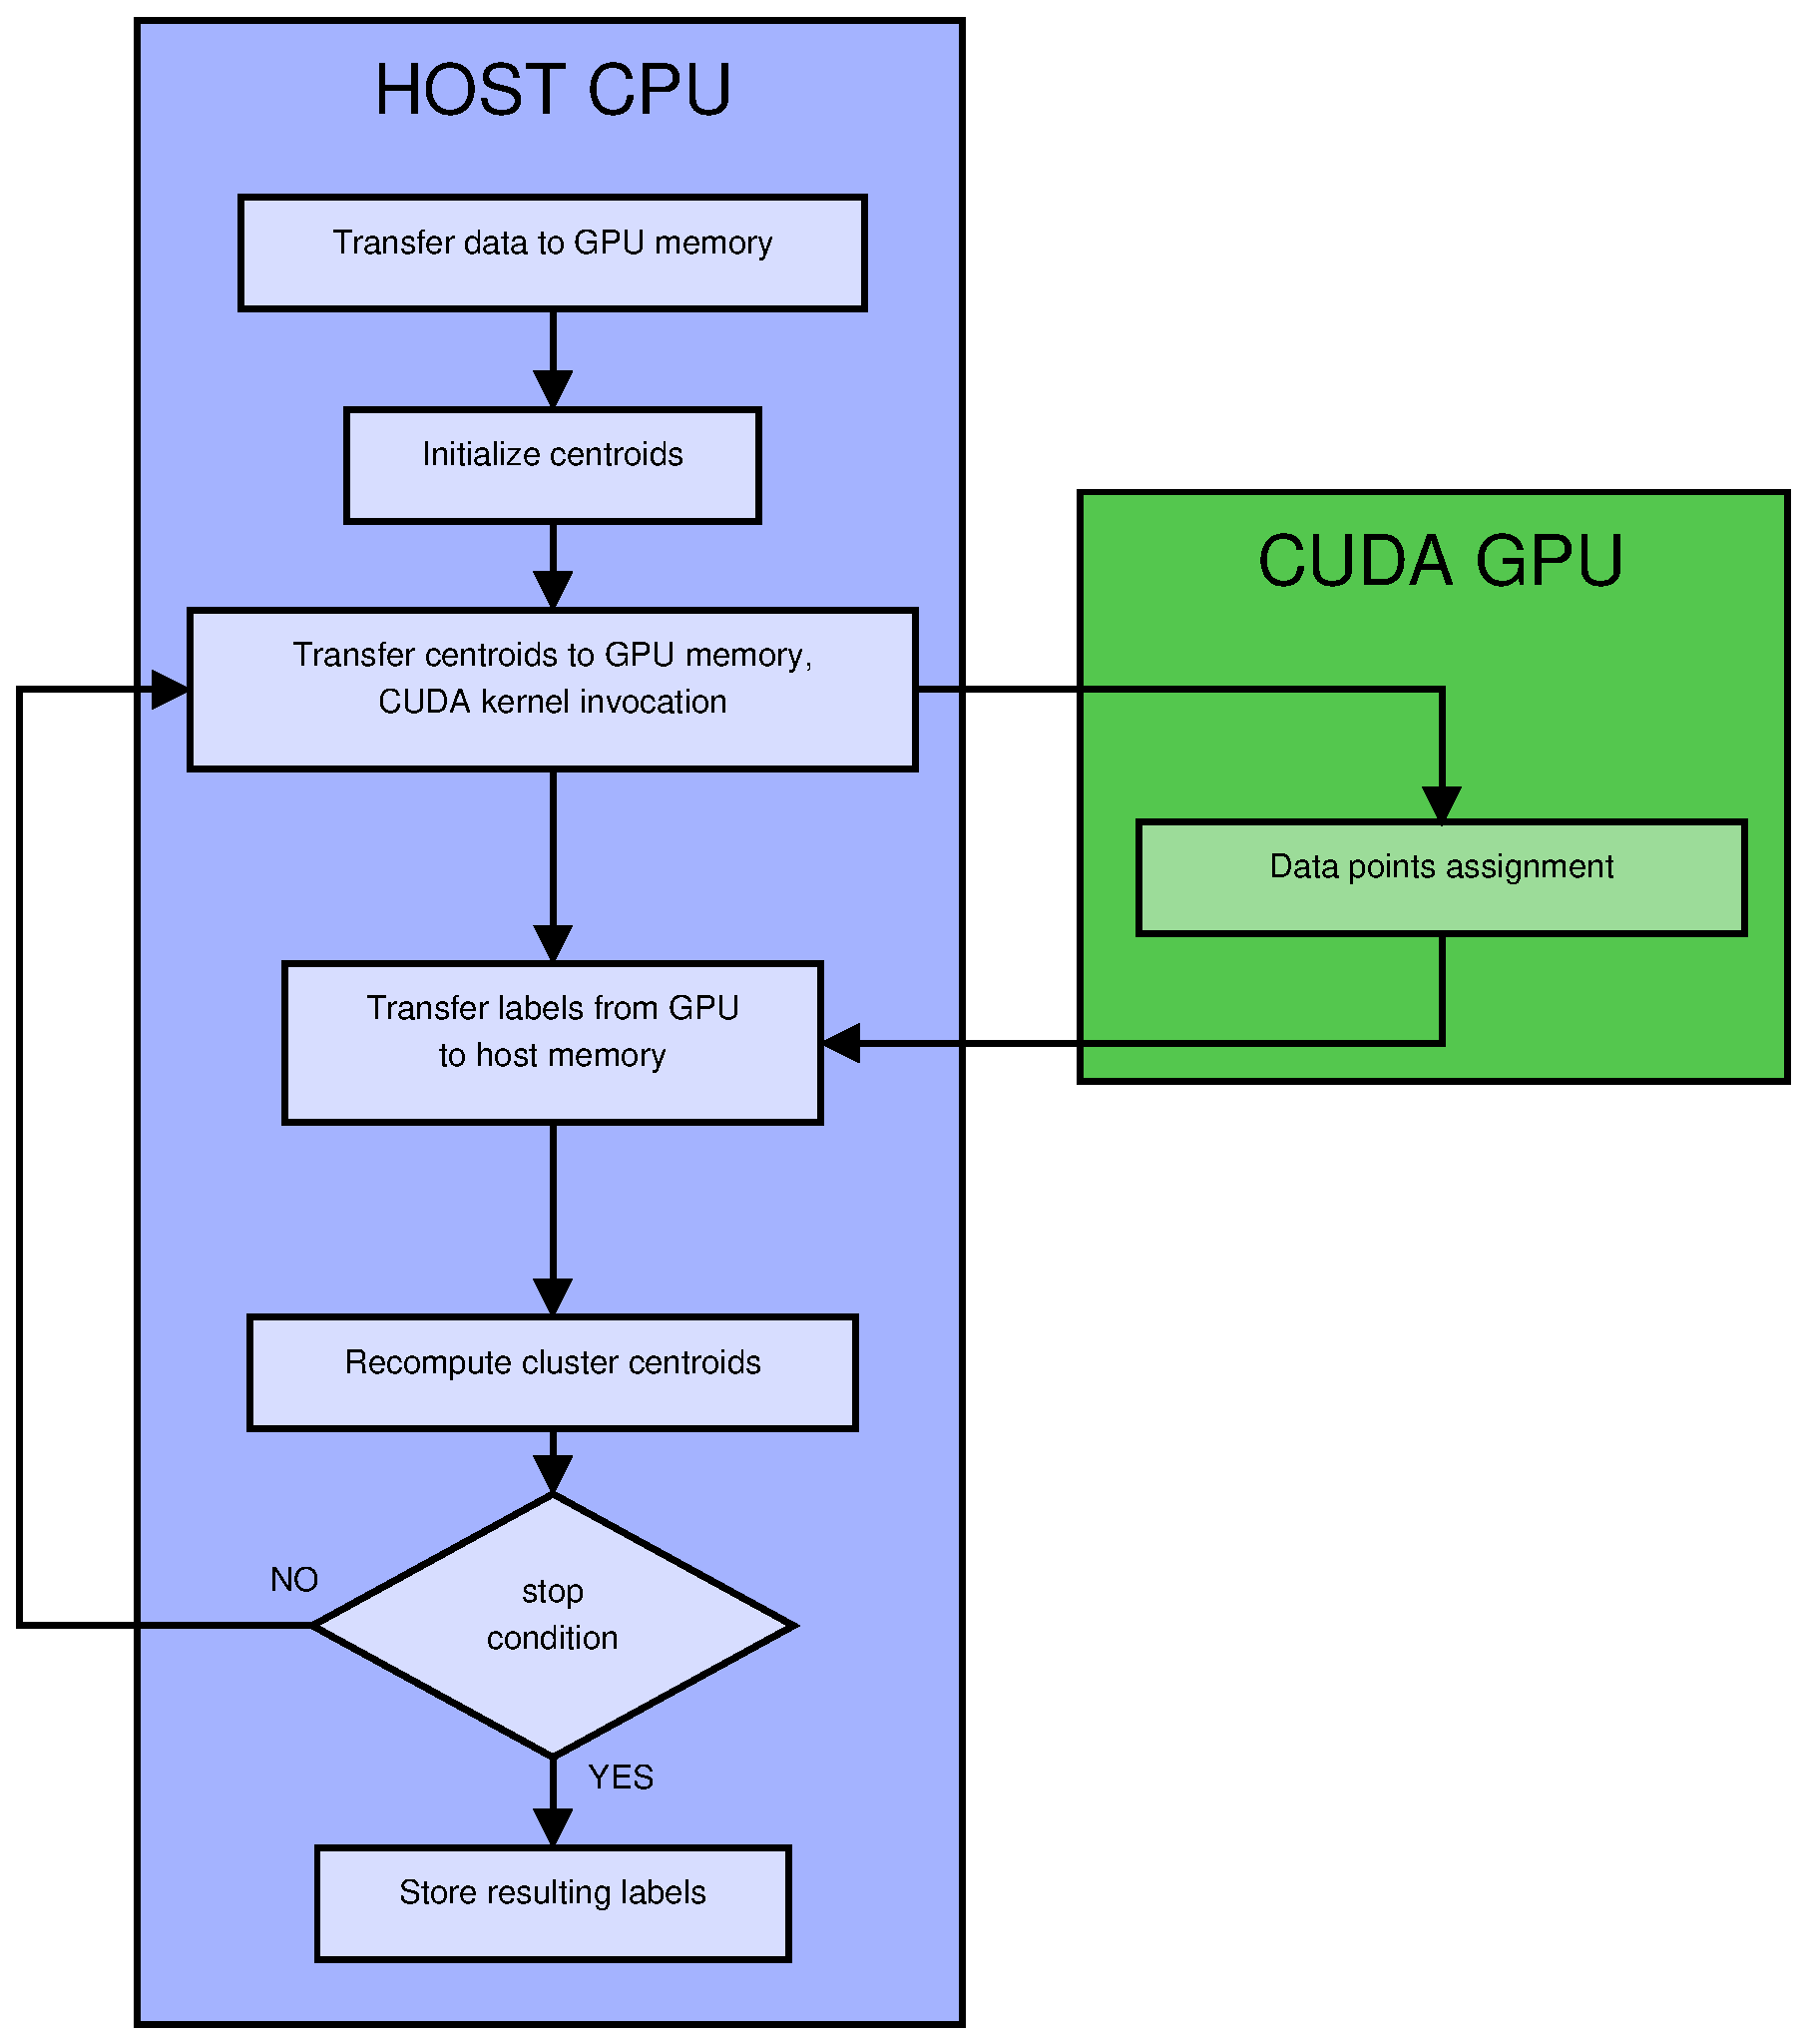
\includegraphics[width=0.7\textwidth]{stateofart/gpgpu/kmeans}
	\caption{Flow execution of the GPU parallel K-Means algorithm.}
	\label{fig:kmeans}
\end{figure}

It should be noted that the literature reports that the performance of K-Means using Dynamic Parallelism is slightly worse than its standard GPU counterpart \cite{DiMarco2013}.
% The results of aforementioned study showed datasets sufficiently large to make them relevant for the present work, considering the focus of the dissertation. 

\subsection{Parallel Single-Link Clustering}

Single-Link (SL) is an important step in the EAC chain.
Given the new similarity metric (how many times a pair of patterns are clustered together in the ensemble), SL provides an intuitive way of obtaining the final partition: patterns that are clustered together often in the ensemble should remain clustered together in the final solution.

% explain how SL works -> is done in the clusteirng chapter
% The sequential SL algorithm works over a pair-wise similarity matrix and starts by considering that every data point is a separate cluster.
% Then, in each iteration, it selects the smallest weight that connects two clusters and merges the two clusters.
% The algorithm stops when $n-1$ merges have been performed, which is when all the data points have been connected in the same cluster.
% The output is a dendrogram connecting all the data points at different levels.

% SL link to MST
SL is not easily parallelized since a new cluster generated at each step may include the one generated in the previous iteration.
The most parallelizable part is the computation of the pair-wise similarity matrix, which is only useful if the input is raw data instead of a similarity matrix as in the case of EAC.
%, which in EAC is computed with the part of the input (the co-association matrix) and, thus, not considered.
The relationship between SL and the Minimum Spanning Tree, explained in chapter \ref{chapter:clustering}, is the key to parallelize it.
If one takes this approach for solving the SL problem, it becomes easier to parallelize it since parallel MST algorithms are abundant in literature \cite{Vineet2009,rostrup2013fast,Sousa2015}.
The same approach for extracting the final clustering in EAC was used in \cite{Fred2002}.

% An important relationship between SL and the Minimum Spanning Tree problem of graphs is the key to parallelize SL.
% If one takes the pair-wise similarity matrix to be a graph (each pattern is a node and each association an edge), then, when performing SL over this graph, the result can be interpreted as a structured MST.
% To get $n$ clusters, one cuts the $n-1$ links with highest cost.
% Furthermore, the MST approach to solve SL has been reported to be among the fastest solutions, since (1) it needs only $O(n)$ working space instead of the $O(n^2$ space of a pair-wise similarity matrix working copy and (2) it reads each similarity only once \cite{Mullner2011}.
% It should be noted that another algorithm with the characteristics mentioned for the MST approach for SL exist in another algorithm, the SLINK \cite{Sibson1973}, which even has some advantages under certain conditions \cite{Mullner2011}.

\subsubsection{Algorithm for finding Minimum Spanning Trees}
There are several algorithms for computing an MST.
The most famous are Kruskal \citep{kruskal1956shortest}, Prim \citep{prim1957shortest} and Borůvka \citep{boruuvka1926jistem}.
Borůvka's algorithm is also known as Sollin's algorithm.
The first two are mostly sequential, while the latter has the highest potential for parallelization, specially in the first iterations.
As such, even though GPU parallel variants of Kruskal's \citep{rostrup2013fast} and Prim's \citep{Wang2011} algorithms exist, the focus will be on Borůvka's.% (which was also the first to be parallelized for the GPU).

Several parallel implementations of this algorithm for the GPU exist, e.g. \citep{Vineet2009}, \cite{harish2009large} and \citep{Sousa2015}. \citet{Sousa2015} provides a more in-depth review over the current state of the art of MST solvers for the GPU and proposes an algorithm reported to be the fastest.
This section will review the algorithm proposed in \citep{Sousa2015}, referred to as \emph{Sousa2015} from henceforth.

\subsubsection{CSR format}
\emph{Sousa2015} takes in a graph as input, represented in the CSR format (a format used for sparse matrices).
This representation is equivalent to having a square matrix $G$ with zeroed diagonal where the $g_{ij}$ element of the matrix is the weight of the link connecting the node $i$ with the node $j$.
This format is represented in Fig. \ref{fig:csr}.
It requires three arrays to fully describe the graph:

\begin{itemize}
	\item a \emph{data} array containing all the non-zero values, where values from the same row appear sequentially from left to right and top to bottom, i.e. in \emph{row-major} order, e.g. if the first row has 20 non-zero values, then the first 20 elements from this array belong to the first row;
	\item a \emph{indices} array of the same size as \emph{data} containing the column index of each non-zero value;
	\item a \emph{indptr} array of the size of the number of rows containing a pointer to the first element in the \emph{data} and \emph{indices} arrays that belongs to each row, e.g. if the $i-th$ element (row) of \emph{indptr} is $k$ and it has 10 values, then all the elements from $k$ to $k + 10$ in \emph{data} belong to the $i-th$ row.
\end{itemize}

\begin{figure}[hbtp]
\centering
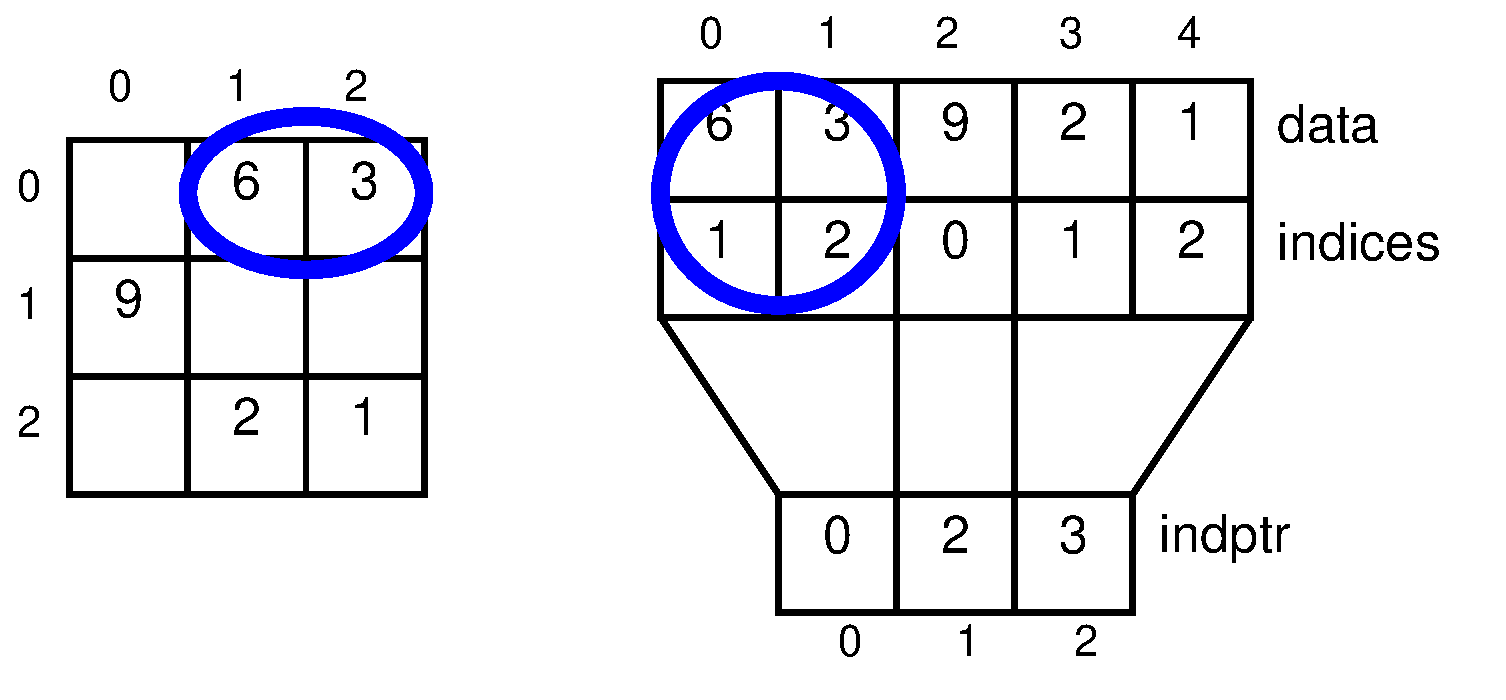
\includegraphics[width=0.5\textwidth]{stateofart/gpgpu/csr_format}
\caption{Correspondence between a sparse matrix and its CSR counterpart.}
\label{fig:csr}
\end{figure}

Within the algorithm's context, these three arrays are denominated as \emph{first\_edge}, \emph{destination} and \emph{weight}, respectively.
There change in denomination is for making their purposes clearer.
Although these three arrays can completely describe a graph, the algorithm uses an extra array \emph{outdegree} that stores the number of non-zero values of each row and can be deduced from the \emph{first\_edge} array.
The length and purpose of each of this arrays are:
\begin{itemize}
	\item \emph{first\_edge} is an array of size $\|V\|$, where the \emph{i-th} element points to the first edge corresponding to the \emph{i-th} edge.
	\item \emph{outdegree} is an array of size $\|V\|$, where the \emph{i-th} element contains the number of edges attached to the \emph{i-th} edge.
	\item \emph{destination} is an array of size $\|E\|$, where the \emph{j-th} element points to the destination vertex of the \emph{j-th} edge.
	\item \emph{weight} is an array of size $\|E\|$, where the \emph{j-th} element contains the weight of the \emph{j-th} edge.
\end{itemize}

$V$ is the number of vertices and $E$ is the number of edges.
The number of edges is duplicated to cover both directions, since the algorithm works with undirected graphs.
This basically means that instead of using the the upper (of lower) triangular matrix (which can also completely describe the graph), it uses the complete one resulting in double redundancy of each edge.
The edges in the \emph{destination} array are grouped together by the vertex they originate from, e.g. if edge $j$ is the first edge of vertex $i$ and this vertex has 3 edges, then edges $\{j,j+1,j+2\}$ are the outgoing edges of vertex $i$.

\subsubsection{Steps of the algorithm}

Within the context of the algorithm the \emph{id} of a vertex is its index in the \emph{first\_edge} array, the \emph{color} is related to the \emph{ids} and the \emph{successor} of a vertex is the destination vertex of one of its edges. The algorithm's flow is represented in Figure \ref{fig:mst sousa} and its main steps are explained below:

\begin{enumerate}
	\item \emph{Find minimum edge per vertex}: select and store the minimum weighted edge for each vertex and resolve same weight conflict by picking the edge with lower destination vertex id.
	\item \emph{Remove mirrored edges}: a mirrored edge the successor of its destination vertex is its origin vertex.
	All mirrored edges are removed from the selected edges in the first step. All edges that are not removed are added to the resulting MST.

	\item \emph{Initialize and propagate colors}: this step is responsible for identifying connected components so the graph may be contracted.
	Each connected component will be a super-vertex in the contracted graph, which means it will be a single vertex that is representing a subgraph.
	Each vertex is initialized with the same color of its successor's id.
	If a vertex has no successor because that edge was removed in the previous step than its color is initialized with its own id.
	The colors are then propagated by setting each vertex's color to the color of its successor, until convergence.

	\item \emph{Create new vertex ids}: only the super-vertices will be propagated to the next iteration but they will have new ids for building the new contracted graph.
	The new ids will range from $0$ to $s$, where $s$ is the number of super-vertices.
	The vertex that will represent a super-vertex is the vertex whose color is its own id.
	The representative vertices will take the new ids in increasing order according to their own ids in increasing order, e.g. vertex $2$ is the representative with lowest id so it will have the id $0$ in the contracted graph.
	This step relied on the \emph{exclusive scan} operation, which is explained in section \ref{sub:scan}.

	\item \emph{Count, assign, and insert new edges}: the final step is where the final operations for building the contracted graph are performed.
	The algorithm will count the number of edges that each super-vertex has connecting to other super-vertices, i.e. the connections between subgraphs.
	This is simply accomplished by selecting every edge whose origin and destination colors are distinct.
	For each such edge the corresponding positions of the origin and destination super-vertices in a new \emph{outdegree} array are incremented with an atomic operation.
	The new \emph{first\_edge} array is obtained from performing an exclusive scan over \emph{outdegree}.
	The next step is to assign and insert edges in the contracted graph.
	Once again, the algorithm will determine which edges will be in the contracted graph by checking the origin and destination colors.
	A copy \emph{top\_edge} of the new \emph{first\_edge} array is done to keep track of where to insert the new edges.
	When an edge is assigned to a super-vertex it is inserted (in the new \emph{weight} and \emph{destination} arrays) in the position specified in \emph{top\_edge} and the algorithm increments \emph{top\_edge} so the next edge will not overwrite the previous one.
	The increment is done with an atomic operation since multiple edges can be assigned to the same super-vertex and the insertion of all edges is being done in parallel.
	It should be noted that duplicated edges are note removed, i.e. several distinct connections between two super-vertices can be kept, since the author considers that the benefit of doing so does not outweigh the computational overhead.
\end{enumerate}

\begin{figure}[hbtp]
\centering
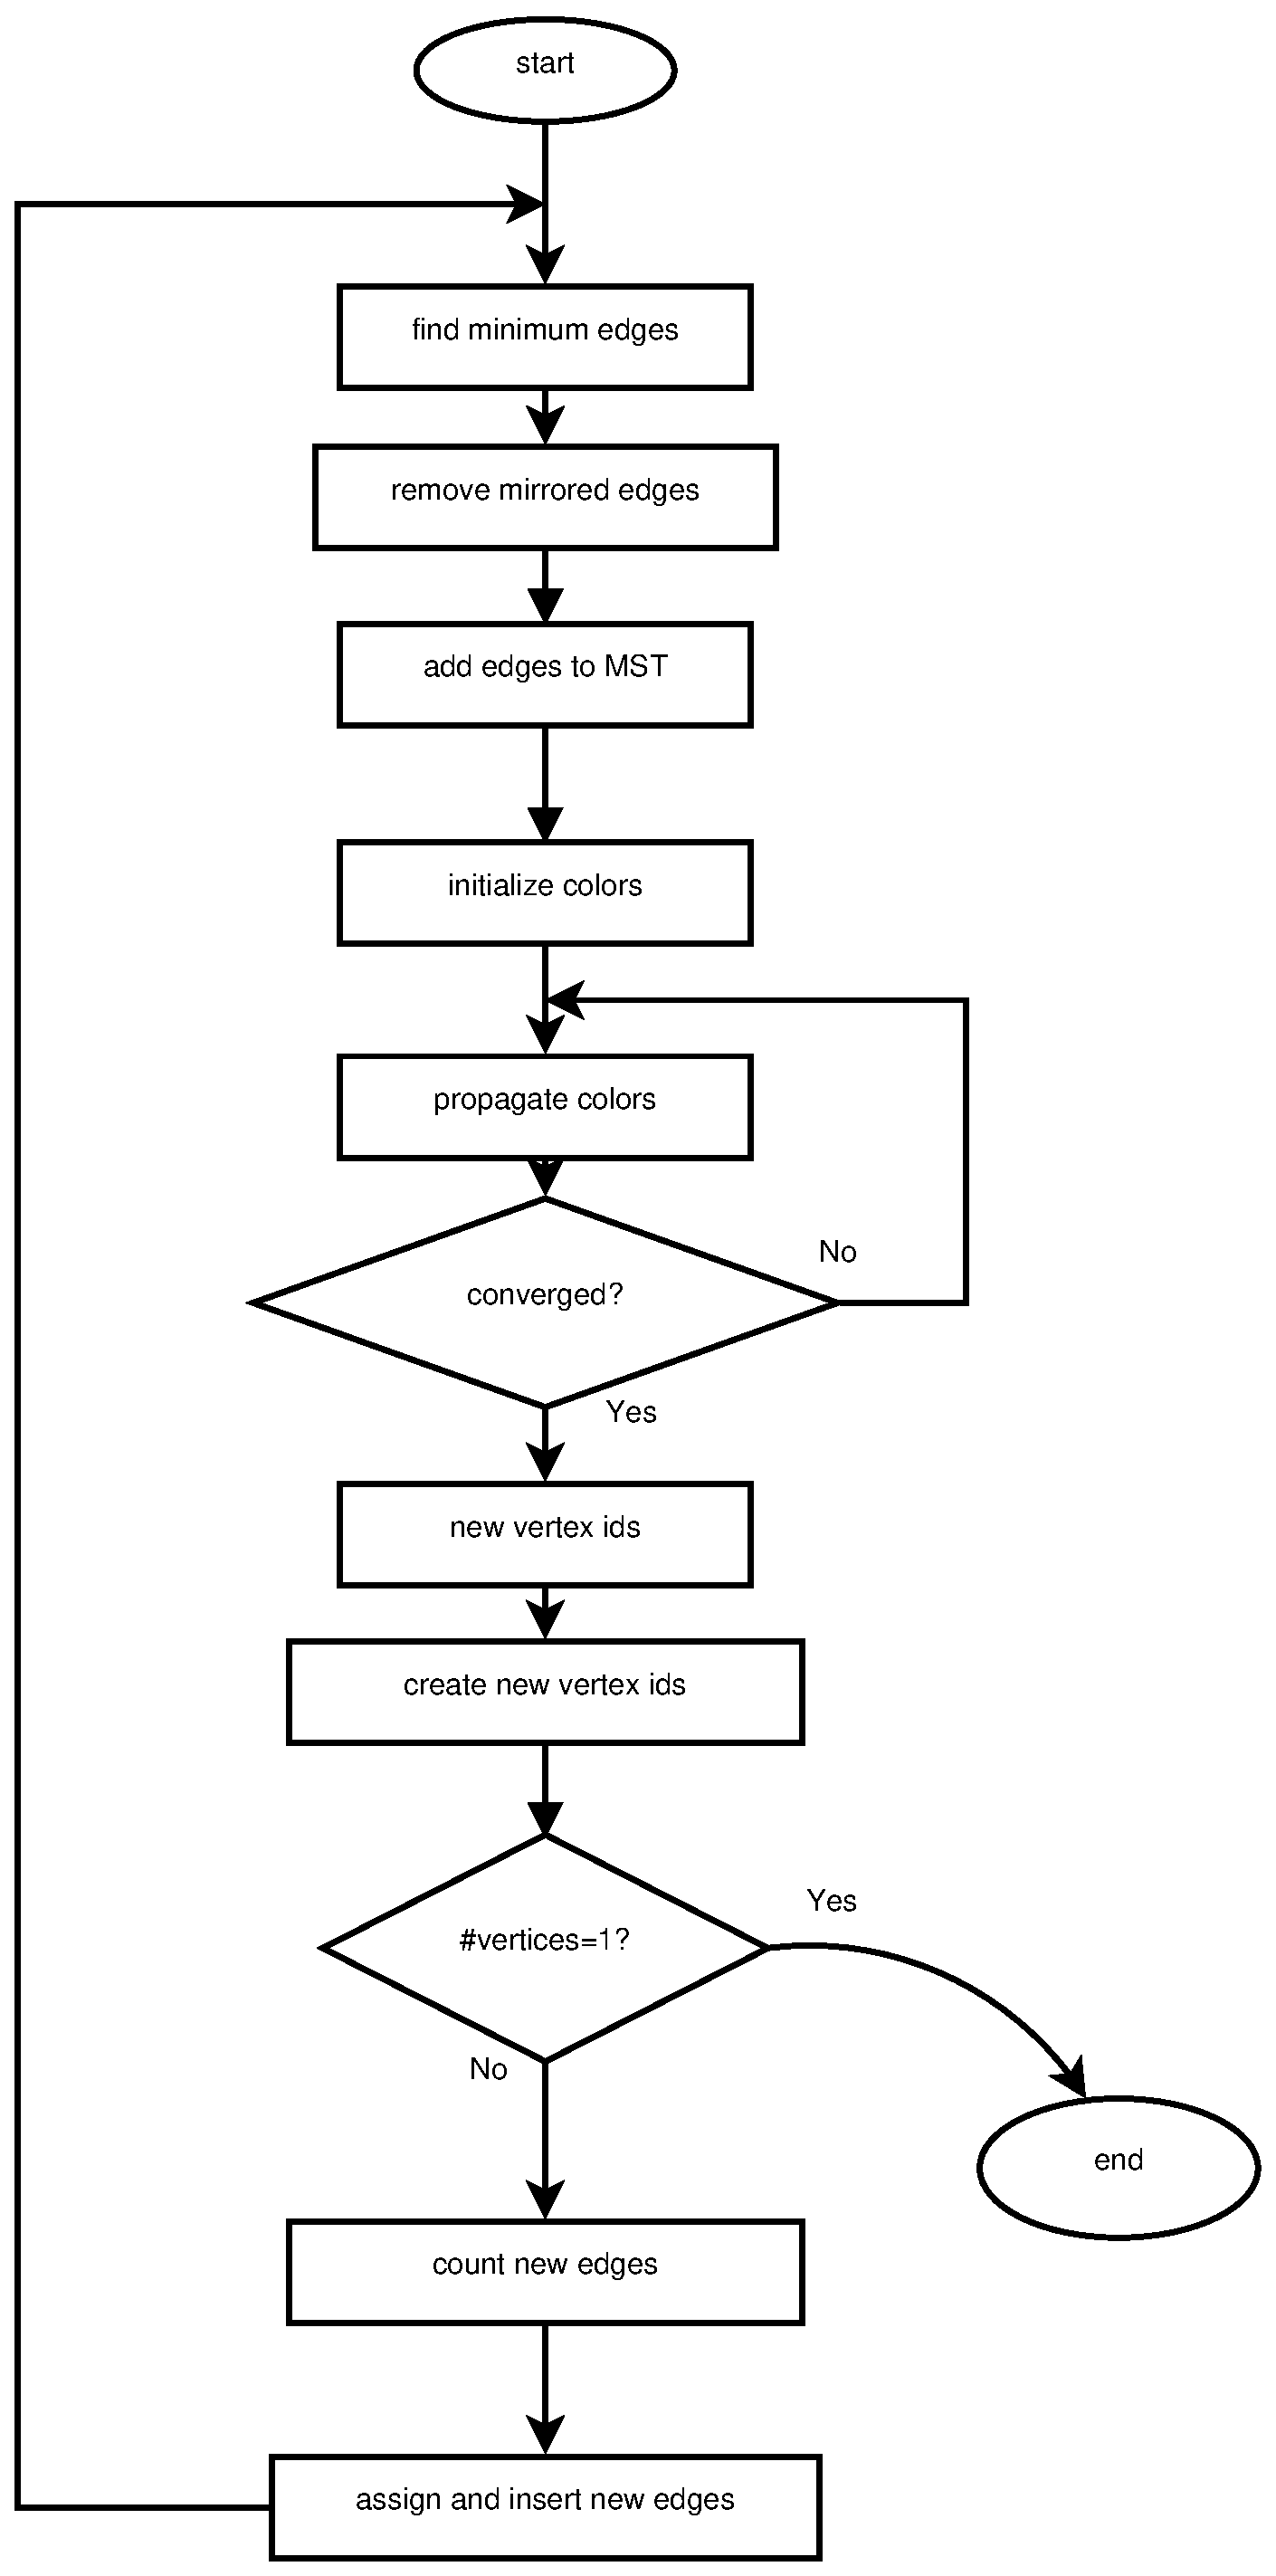
\includegraphics[width=0.5\textwidth]{stateofart/gpgpu/mst_boruvka_flow}
\caption{Flow execution of Sousa2015.}
\label{fig:mst sousa}
\end{figure}

It should be noted, however, that this algorithm doe not support unconnected graphs, i.e., it is not able to output a forest of MSTs.
Upon contact, the author reported that a solution to that problem is, on the step of building the flag array, only mark a vertex if it is both the representative of its supervertex and has at least one neighbour.

\subsubsection{Exclusive scan}
\label{sub:scan}
%Algorithm 1 assumes that there are as many processors as data elements. For large arrays on a GPU running CUDA, this is not usually the case. Instead, the programmer must divide the computation among a number of thread blocks that each scans a portion of the array on a single multiprocessor of the GPU. Even still, the number of processors in a multiprocessor is typically much smaller than the number of threads per block, so the hardware automatically partitions the "for all" statement into small parallel batches (called warps) that are executed sequentially on the multiprocessor. An NVIDIA 8 Series GPU executes warps of 32 threads in parallel. Because not all threads run simultaneously for arrays larger than the warp size, Algorithm 1 will not work, because it performs the scan in place on the array. The results of one warp will be overwritten by threads in another warp.

%To solve this problem, we need to double-buffer the array we are scanning using two temporary arrays. Pseudocode for this is given in Algorithm 2, and CUDA C code for the naive scan is given in Listing 39-1. Note that this code will run on only a single thread block of the GPU, and so the size of the arrays it can process is limited (to 512 elements on NVIDIA 8 Series GPUs). Extension of scan to large arrays is discussed in Section 39.2.4.

The \emph{scan} operation is one of the fundamental building block of parallel computing. 
Furthermore, two of the steps of the Borůvka variant of \cite{Sousa2015} are performed with an exclusive scan where the operation is a sum. 
To illustrate the functioning of the exclusive scan, let us consider the particular case where the operation of the scan is the sum and the identity (the value for which the operation produces the same output as the input) is naturally $0$.
Let us further consider the input array to be the sequence $[0,1,2,3,4,5,6,7]$.
Then the output will be $[0,0,1,3,5,8,13,19]$.
The first element of the output will be the identity (if it were an inclusive scan, it would be the first element itself).
The second element is the sum between the first element of the input array and the first element of the output array, the third element is the sum between the second element of the input array with second element of the output array, and so on.
This algorithm seems highly sequential in nature each element of the output array depends on the previous one, but two main parallel versions can be found in literature: Hillis and Steele's \cite{Hillis1986} and Blelloch's \cite{Blelloch1990}. 
The two approaches focus on distinct efforts: the former focus on optimizing the number of steps \cite{Hillis1986} while the latter focus on optimizing the amount of work done \cite{Blelloch1990}.
The focus will be on the Blelloch's algorithm.

Blelloch's algorithm is comprised by two main phases: the \emph{reduce phase} (or \emph{up-sweep}) and the \emph{down-sweep phase}.
The algorithm is based on the concept of \emph{balanced binary trees} \cite{Harris2007}, but it should be noted that no such data structure is actually used.
An in-depth explanation of this concept and how it relates to the algorithm being reviewed falls outside the scope of the present work and it is recommended that the reader consult \cite{Harris2007} or \cite{Blelloch1990} for such details.

During the reduce phase (see Figure \ref{fig:scan reduce}), the algorithm traverses the tree and computes partial sums at the internal nodes of the tree.
This operation is also known as a parallel reduction due to the fact that the total sum is stored in the root node (last node) of the tree \cite{Harris2007}.

\begin{figure}[hbtp]
\centering
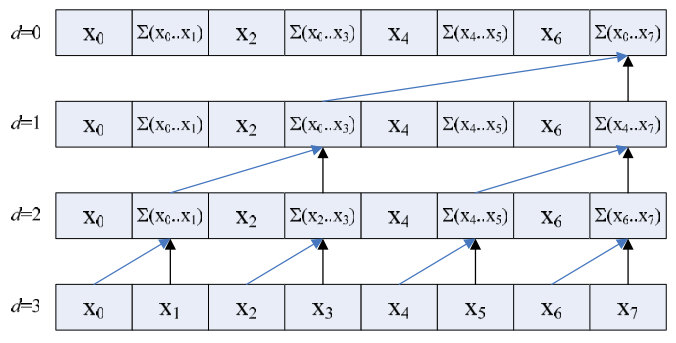
\includegraphics[width=0.8\textwidth]{stateofart/gpgpu/blelloch_reduce}
\caption{Representation of the reduce phase of Blelloch's algorithm \cite{Harris2007}. \emph{d} is the level of the tree and the input array can be observed at $d=0$.}
\label{fig:scan reduce}
\end{figure}

In the down-sweep phase (see Figure \ref{fig:scan down-sweep}) the algorithm traverses back the tree.
During the traversal, and using the partial sums calculated in the reduce phase, it builds the scan in place (overwriting the result of the reduce phase).

\begin{figure}[hbtp]
\centering
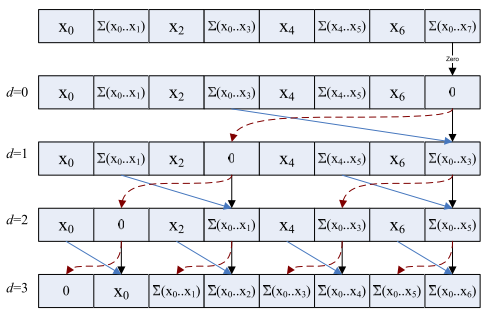
\includegraphics[width=0.8\textwidth]{stateofart/gpgpu/blelloch_downsweep}
\caption{Representation of the down-sweep phase of Blelloch's algorithm \cite{Harris2007}. \emph{d} is the level of the tree.}
\label{fig:scan down-sweep}
\end{figure}

This the computational complexity of this algorithm is higher than that of its sequential counterpart.
The sequential version has a $O(n)$ computational complexity since it only goes through the input array once and performs exactly $n$ additions.
Blelloch's algorithm, in the other hand, performs $2(n-1)$ additions in the reduce phase and $n-1$ swaps in the down-sweep phase.
However, since it is a parallel algorithm and the computation will be distributed across several processing units, it still performs better.
It should also be noted that, as described, the algorithm supports input arrays of a size that is a power of $2$.
However, \cite{Harris2007} explains how to overcome this limitation and also offers an implementation for CUDA and hardware specific optimizations.

% % % % % % % % % % % % % % % % % % % % % % % % % % % % % % % % % % % % % % % %
%
%  					QUANTUM CLUSTERING
%
% % % % % % % % % % % % % % % % % % % % % % % % % % % % % % % % % % % % % % % %

\section{Quantum clustering}
\label{sec:quantum clustering}
% double check all refs because this was merged pre latex citations and the reference might have gotten mixed

% TODO add more refs for quantum inspired computational intelligence; Applications of quantum inspired computational intelligence: A survey is good article to take stuff from

The field of quantum clustering has shown promising results regarding potential speed-ups in several tasks over their classical counterparts. 
Currently, two major approaches for the concept of quantum clustering were found in the literature: quantization quantization of clustering methods to work in quantum computers or algorithms inspired by quantum physics.

The former approach translates in converting algorithms to work partially or totally on a different computing paradigm, with support of quantum circuits or quantum computers.
% relevant papers for machine learnigng quantum paradigm
Both \citet{Aimeur2013} and \citet{Lloyd2013} show how the quantum paradigm can be used for speed-ups in the machine learning algorithms, with the possibility of obtaining exponential speed-ups.
Many of these quantizations make use of Groover's database search algorithm \cite{grover1996fast}, or a variant of it, e.g. \citet{Wiebe2014}.
Most literature on this approach is also mostly theoretical, since the physical requirements still do not exist for testing these methods.
This approach can be seen as part of the bigger problem of quantum computing and quantum information processing.
An alternative to using real quantum systems would be to simulate them.
% get refs for simulation of quantum systems not being feasable; Feynmann; I think washington course had something
However, simulating quantum systems in classical computers is a very hard task by itself and literature suggest that it is not feasible \cite{Feynman1982}.
% Given that the scope of the thesis is to accelerate clustering, having the extra overhead of simulating the systems would not allow speed-ups. 
The quantization approach falls outside the scope of this dissertation, but \citet{wittek2014quantum} offers a thorough review on the state of the art of machine learning in the quantum paradigm.

% Computational intelligence is the second approach, i.e. to use algorithms that muster inspiration from quantum analogies.
The second approach is part of the wider field of Computational Intelligence.
A study of the literature reveals that it typically further divides itself into two categories \cite{Casper2013}.%, depending on which concept the algorithm is based: the quantum bit or Schrödinger's wave equation.
One comprises the algorithms based on the concept of the qubit, the quantum analogue of a classical bit with interesting properties found in quantum objects.
Several algorithms have been modeled after this concept, often also gathering inspiration from evolutionary genetic algorithms, which were successfully applied in several areas:
\begin{itemize}
	\item tackling the Knapsack problem as described in \citet{Han2000} and its improved version \cite{Liu2010};

	\item solving the traveling salesman problem \cite{Talbi2004};

    \item two implementations of a Quantum K-Means algorithm \cite{Casper2012KMeans,Xiao2010};

    \item a Quantum Artificial Bee Colony algorithm \cite{hung2013quantum,Casper2013};

    \item two approaches for Fuzzy C-Means (FCM), namely Quantum New Weighted Fuzzy C-Means (QNW-FCM) \cite{Casper2013} and Quantum Fuzzy C-Means (QFCM) \cite{hung2013quantumcmeans,Casper2013};

    \item a novel quantum inspired clustering technique based on manifold distance \cite{Liang2009};

    \item a Quantum-inspired immune clonal clustering algorithm based on watershed \cite{Li2010}.
\end{itemize}

%schrodinger
The other approach models data as a quantum system and uses Schrödinger's equation in some way.
Often, the data is modeled as a quantum system, where each pattern is a particle, and Schrödinger's equation is used to evolve the particle system into a solution.
This has been applied in an optimization problem for electromagnetics using a quantum particle swarm \cite{mikki2006quantum} and also on several clustering algorithms:
\begin{itemize}
	\item the Quantum Clustering \cite{Horn2001b} algorithm treats patterns as quantum particles whose potential is computed with Schrödinger's equation and the system is evolved with the Gradient Descent method;

	\item Dynamic Quantum Clustering \cite{Weinstein2009b} is a variation of \citet{Horn2001b} that uses Schrödinger's equation to evolve the system;

	\item a Fuzzy C-Means approach \cite{li2007quantum} based on Quantum Clustering \cite{Horn2001b};

	\item QPSO+FCM, a Fuzzy C-means \cite{Wang2007} based on Quantum-behaved Particle Swarm Optimization (QPSO) \cite{Sun2004}.

\end{itemize}

For more information on quantum inspired algorithms, the reader is referred to \citet{Manju2014} which offers a thorough survey on the state of the art of quantum inspired computation intelligence algorithms.
The following two sections contain a brief overview of the concept of the qubit and the description of an algorithm that uses this approach.
Afterwards, an algorithm that follows the Schrödinger's equation approach is reviewed.

\subsection{The quantum bit approach}
\label{sec:qubit}

\subsubsection{The quantum bit}

To understand the algorithms based on the concept of the qubit, it is useful to cast some insight about its properties and functioning.
This section has the purpose to provide a brief introduction to this topic.
An extended and in-depth review of this and related topics can be found in \citet{Lanzagorta2008}.
The qubit is a quantum object with certain quantum properties such as entanglement and superposition.
Within the context of the studied algorithm, the only property used is superposition.
A qubit can have any value between 0 and 1 (superposition property) until it is observed, which is when the system collapses to either state.
However, the probability with which the system collapses to either state  may be different.
The superposition property or linear combination of states can be expressed \cite{Casper2012KMeans} as % add ref for the mathematical formulation below: this can be found in the QK-Means papers


$$
% [\psi] = \alpha[0] + \beta[1]
| \psi \rangle = \alpha | 0 \rangle + \beta | 1 \rangle
$$

where $\psi$ is an arbitrary state vector and $\alpha$, $\beta$ are the the probability amplitude coefficients of basis states $| 0 \rangle$ and $| 1 \rangle$, respectively.
The Dirac bra ket notation is employed, where the \emph{ket} $| . \rangle$ corresponds to a column vector.
The basis states correspond to the spin of the modeled particle (in this case, a ferminion, e.g. electron).
The coefficients are subjected to the following normalization:

$$|\alpha|^2 + |\beta|^2 = 1$$

where $|\alpha|^2$, $|\beta|^2$ are the probabilities of observing states $[0]$ and $[1]$, respectively. $\alpha$ and $\beta$ are complex quantities and represent a qubit:

$$\begin{bmatrix}
\alpha \\
\beta
\end{bmatrix}$$

Moreover, a qubit string may be represented by:
$$
\begin{bmatrix}
\left. \begin{matrix}
\alpha_1\\ 
\beta_1
\end{matrix}\right| & \left.\begin{matrix}
\alpha_2\\ 
\beta_2
\end{matrix}\right| & \begin{matrix}
\alpha_3\\ 
\beta_3
\end{matrix}
\end{bmatrix}
$$

The probability of observing the state $|000 \rangle$ will be $|\alpha_1|^2 \times |\alpha_2|^2 \times |\alpha_3|^2$.
To use this model for computing purposes, black-box objects called \emph{oracles} are used.
Oracles are important to understand quantum speed-ups.
They can be understood as subroutines that cannot be usefully examined or as unknown physical systems that perform a quantum operation on a qubit string \cite{Rosenbaum2011} and with properties one would like to estimate.
Within the context of the present work an oracle is an abstraction for the programmer.
It is an object which can be called and changes state (which can be observed) as a consequence.
For the purpose of the following sections, the concept of the oracle is more related to \emph{oracles with internal randomness} \cite{Rosenbaum2011} or, more simply, a probabilistic Turing machine, as in the case of \cite{hung2013quantum}.

% # get ref -->
% Def from wiki: In complexity theory and computability theory, an oracle machine is an abstract machine used to study decision problems.
% It can be visualized as a Turing machine with a black box, called an oracle, which is able to decide certain decision problems in a single operation.
% The problem can be of any complexity class.
% Even undecidable problems, like the halting problem, can be used. %from http://en.wikipedia.org/wiki/Oracle_machine


\subsubsection{Quantum K-Means}
\label{sec:qkmeans}

% Several clustering algorithms \cite{Casper2013,Casper,Xiao2010}, as well as optimization problems \cite{Wang2013}, are modeled after this concept.
% To test the potential of the algorithms under this paradigm, a quantum variant of the K-Means algorithm based on\cite{Casper} was chosen as a case study.

% This section will describe the Quantum K-Means algorithm \cite{Casper2012KMeans}.


% \subsubsection{Description of the algorithm}

The Quantum K-Means (QK-Means) algorithm, as described in \cite{Casper2012KMeans}, is based on the classical K-Means algorithm.
It extends the basic K-Means with concepts from quantum mechanics (the qubit) and evolutionary genetic algorithms.

Within the context of this algorithm, oracles contain strings of qubits and generate their own input by observing the state of the qubits.
After collapsing, the qubit value corresponds to a classical bit, with a binary value.

Ideally, oracles would contain actual quantum systems or simulate them - this would correctly account for the desirable quantum properties.
As it stands, oracles are not quantum systems or even simulate them and can be more appropriately described as random number generators.
Each string of qubits represents a number, so the number of qubits in each string will define its precision.
The number of strings chosen for the oracles depends on the number of clusters and dimensionality of the problem (e.g. for 3 centroids of 2 dimensions, 6 strings will be used since 6 numbers are required).
Each oracle will represent a possible solution.

The algorithm has the following steps:
\begin{enumerate}
\item Initialize population of oracles
\item Collapse oracles
\item K-Means
\item Compute cluster fitness
\item Store
\item Quantum Rotation Gate
\item Collapse oracles
\item Quantum cross-over and mutation
\item Repeat 3-7 until generation (iteration) limit is reached
\end{enumerate}


\paragraph{Initialize population of oracles}

The oracles are created in this step and all qubit coefficients are initialized with $\frac{1}{\sqrt{2}}$, so that the system will observe either state of the qubit with equal probability.
This value is chosen taken into account the necessary normalization of the coefficients, as described in the previous section.

\paragraph{Collapse oracles}

Collapsing the oracles implies making an observation of every qubit of each string in all oracles.
This is done by first choosing a coefficient to use (either can be used), e.g. $\alpha$.
Then, a random value $r$ between 0 and 1 is generated.
If $\alpha \ge r$ then the system collapses to $[0]$, otherwise to $[1]$.

\paragraph{K-Means}
In this step we convert the binary representation of the qubit strings to base 10 and use those values as initial centroids for K-Means.
For each oracle, classical K-Means is then executed until it stabilizes or reaches the iteration limit.
The solution centroids are returned to the oracles in binary representation.

\paragraph{Compute cluster fitness}
Cluster fitness is computed using the Davies-Bouldin index for each oracle.
The score of each oracle is stored in the oracle itself.

\paragraph{Store}
The best scoring oracle is stored.

\paragraph{Quantum Rotation Gate}
So far, the algorithm consisted of the classical K-Means with a complex random number generation for the centroids and complicated data structures, namely the oracles.
This is the step that fundamentally differs from the classical version.
In this step, a quantum gate (in this case a rotation gate) is applied to all oracles except the best one.
The basic idea is to shift the qubit coefficients of the least scoring oracles in the direction of the best scoring one.
These oracles will have a higher probability of collapsing into initial centroid values closer to the best solution so far.
This way, in future generations, the oracles do not initiate with the best centroids so far (which would not converge into a better solution) but we they are close while still ensuring diversity (which is also a desired property in the genetic computing paradigm).
In other words, we look for better solutions than the one we got before in each oracle while moving in the direction of the best we found so far.

The genetic operations of cross-over and mutation are both part of the genetic algorithms toolbox.
Literature suggests that this operations may not be required to produce variability in the population of qubit strings \cite{Liu2010}.
The reason for this is that enough variability is produced with the use of the angle-distance rotation method \cite{Liu2010} in the quantum rotation operation, with a careful choice of the rotation angle.
Still, when used, the goal of these operations is to produce further variability into the population of qubit strings.

\subsection{Schrödinger's equation approach} % Horn and Gottlieb's algorithm}
\label{sec:horn}

The other approach to clustering that gathers inspiration from quantum mechanical concepts is to use the Schrödinger equation.
The algorithm under study was created by Horn and Gottlieb \cite{Horn2010} and was later extended by Weinstein and Horn \cite{Weinstein2009}.

The first step in this methodology is to compute a probability density function of the input data.
This is done with a Parzen-window estimator in \cite{Horn2001a,Weinstein2009}.
The Parzen-window density estimation of the input data is done by associating a Gaussian with each point, such that

$$ \psi (\mathbf{x}) = \sum ^N _{i=1} e^{- \frac{\left \| \mathbf{x}-\mathbf{x}_i \right \| ^2}{2 \sigma ^2}} $$

where $N$ is the total number of points in the dataset, $\sigma$ is the variance and $\psi$ is the probability density estimation. $\psi$ is chosen to be the wave function in Schrödinger's equation.
%The details of why this is fall outside of the scope of the present work and are explained in \cite{Weinstein2009,Horn2001a,Horn2001b}.
Further detals can be found in \citet{Weinstein2009,Horn2001a,Horn2001b}.

With this information, one will compute the potential function $V(x)$ that corresponds to the state of minimum energy (ground state = eigenstate with minimum eigenvalue) \cite{Horn2001a}, by solving the Schrödinger's equation in order of $V(x)$:      

\begin{align}

V(\mathbf{x}) = E + \frac {\frac{\sigma^2}{2}\nabla^2 \psi }{\psi} 
= E - \frac{d}{2} + \frac {1}{2 \sigma^2 \psi} \sum ^N _{i=1} \left \| \mathbf{x}-\mathbf{x}_i \right \| ^2 e^{- \frac{\left \| \mathbf{x}-\mathbf{x}_i \right \| ^2}{2 \sigma ^2}}
\label{eq:wave}
\end{align}

And since the energy should be chosen such that $\psi$ is the groundstate (i.e. eigenstate corresponding to minimum eigenvalue) of the Hamiltonian operator associated with Schrödinger's equation (not represented above), the following is true

\begin{align}
E = - min \frac {\frac{\sigma^2}{2}\nabla^2 \psi }{\psi}
\label{eq:wave sol}
\end{align}

From equations \ref{eq:wave} and \ref{eq:wave sol}, $V(x)$ can be computed.
This potential function is related to the inverse of a probability density function.
Minima of the potential correspond to intervals in space where points are together.
So minima will naturally correspond to cluster centers \cite{Horn2001a}.
However, it is very computationally intensive to compute $V(x)$ to the whole space, so the compututation of the potential function is only done at the data points.
This should not be problematic since clusters' centers are generally close to the data points themselves. 
Even so, the minima may not lie on the data points themselves.
One method to address this problem is to compute the potential on the input data and converge this points toward some minima of the potential function.
This is done with the gradient descent method in \cite{Horn2001a}. 

Another method \cite{Weinstein2009} is to think of the input data as particles and use the Hamiltonian operator to evolve the quantum system in the time-dependent Schrödinger's equation.
Given enough time steps, the particles will converge to and oscillate around potential minima.
This method makes the Dynamic Quantum Clustering algorithm.
The nature of the computations involved in this algorithm make it a good candidate for parallelization techniques.
\citet{Wittek2013} parallelized this algorithm to the GPU obtaining speed-ups of up to two magnitudes relative to an optimized multicore CPU implementation. %TODO: leave this or not? I did not test this so maybe it is better not

% #TODO describe the fine cluster algorithm; critique how this is done; what was developed;

%[1] N. Wiebe, A. Kapoor, and K. Svore, “Quantum Algorithms for Nearest-Neighbor Methods for Supervised and Unsupervised Learning,” p. 31, 2014.
%
%\cite{Wiebe2014}

%[2] D. Horn and A. Gottlieb, “The Method of Quantum Clustering.,” NIPS, no. 1, 2001.
%\cite{Horn2001a}

%[3] M. Weinstein and D. Horn, “Dynamic quantum clustering: a method for visual exploration of structures in data,” Phys. Rev. E - Stat. Nonlinear, Soft Matter Phys., vol. 80, no. 6, pp. 1–15, Dec. 2009.
%\cite{Weinstein2009}

%[4] E. Casper and C. Hung, “Quantum Modeled Clustering Algorithms for Image Segmentation,” vol. 2, no. March, pp. 1–21, 2013.
%\cite{Casper2013}
%
%[5] E. Casper, C.-C. Hung, E. Jung, and M. Yang, “A Quantum-Modeled K-Means Clustering Algorithm for Multi-band Image Segmentation.” [Online]. Available: http://delivery.acm.org/10.1145/2410000/2401639/p158-casper.pdf?ip=193.136.132.10&id=2401639&acc=ACTIVE SERVICE&key=2E5699D25B4FE09E.F7A57B2C5B227641.4D4702B0C3E38B35.4D4702B0C3E38B35&CFID=476955365&CFTOKEN=55494231&__acm__=1423057410_0d77d9b5028cb3. [Accessed: 04-Feb-2015].

%\cite{Casper}

%[6] J. Xiao, Y. Yan, J. Zhang, and Y. Tang, “A quantum-inspired genetic algorithm for k-means clustering,” Expert Syst. Appl., vol. 37, pp. 4966–4973, 2010.
%\cite{Xiao2010}

%
%[7] H. Wang, J. Liu, J. Zhi, and C. Fu, “The Improvement of Quantum Genetic Algorithm and Its Application on Function Optimization,” vol. 2013, no. 1, 2013.
%\cite{Wang2013}

%
%[8] W. Liu, H. Chen, Q. Yan, Z. Liu, J. Xu, and Y. Zheng, “A novel quantum-inspired evolutionary algorithm based on variable angle-distance rotation,” 2010 IEEE World Congr. Comput. Intell. WCCI 2010 - 2010 IEEE Congr. Evol. Comput. CEC 2010, 2010.
%\cite{Liu2010}